\documentclass[a4paper,12pt]{article}

\usepackage{graphicx}	% Pour importer des images
\usepackage[left=2.5cm,right=2.5cm,top=2cm,bottom=3.5cm]{geometry} %Configuration de la page
\usepackage{amsmath}
\usepackage{amsthm}
\usepackage{hyperref}
\usepackage{float}
\usepackage{booktabs}
\usepackage[T1]{fontenc}
\usepackage[table]{xcolor}
\usepackage{tikz}
\usepackage{pgfplots}
\pgfplotsset{compat=1.18}
\usepackage{readarray}
\readarraysepchar{,}

\newtheorem*{remark}{Remark}


\begin{document}

\title{Note on Hypotension Prediction}

\author{Bob Aubouin--Pairault}
\maketitle


\section{Goal of the document}

The goal of this document is to summarize all the work done on the hypotension prediction.


\section{Abstract sent to the conference}

Intraoperative hypotension (IOH) is common during surgical procedures. It may be caused by anesthesia drugs, underlying  comorbidities of the patient such as heart failure, or by the surgical procedure. There are strong associations between IOH and postoperative organ complications, thus the ability to predict IOH to support the clinician is an attractive prospect. In this presentation, the prediction of hypotension during general anesthesia using physiological signal is investigated. \medskip

Recently, some research has been focused on trying to predict hypotension events occurring during surgeries using machine learning techniques \cite{hatibMachinelearningAlgorithmPredict2018}. However, this methodology has been subject to some questioning \cite{enevoldsenPerformanceHypotensionPrediction2022}, \cite{smithConHypotensionPrediction2023}. Especially, the database seems to be biased, and the evaluations are not compared to a relevant baseline. A new methodology addressing the arisen questions is proposed here. Exploratory investigations are illustrated using the open source VitalDB database \cite{leeVitalDBHighfidelityMultiparameter2022} and standard machine learning algorithms. In addition, the explainability of the prediction is studied to provide more information to the anesthesiologist.


\section{Feature selection}

To select the features that are used to predict hypotension, the signals related to blood presure where first considered (mean, systolic, and diastolic blood pressure). Then, the other signals available in the database were considered, heart rate was added as it is obviously related to blood pressure. Then, the respiratory rate, oxygen saturation and the end tidal CO2 were added to represent the respiratory function of the patient. Finally, the hypnotic drug where added as it is known to cause hypotension, we considered the MAC value and the propofol target. We do not consider the raw signals of arterial blood pressure and heart rate as this is a preliminary work. Nevertheless, the use of features extracted from those signals could be of great interest. \medskip

For the static features, the age, the BMI, the ASA, and the hypertension status of the patient were considered. Moreover, the preoperative
creatinine concentration in the blood was added as it is known to be related to the risk of hypotension \cite{owensArterialHypotensionPrevalence2000a}. Other feature such as smoking and alcoholic habits could be of great interest but where not available in the dataset. \medskip
\begin{table}
\small
\begin{center}
\center
\rowcolors{2}{white}{gray!20}
\begin{tabular}{p{0.17\textwidth}|p{0.4\textwidth}|c|c}
\textbf{Feature} & \textbf{Description} & \textbf{VitalDB Name} & \textbf{Code name} \\
\midrule
Mean Arterial Pressure & Average blood pressure during a cardiac cycle & Solar8000/ART\_MBP & mbp\\
Systolic Blood Pressure & Maximum blood pressure during a cardiac cycle & Solar8000/ART\_SBP & sbp \\
Diastolic Blood Pressure & Minimum blood pressure during a cardiac cycle & Solar8000/ART\_DBP & dbp \\
Heart Rate & Number of heart beats per minute & Solar8000/HR & hr\\
Respiration Rate & Number of breaths per minute & Solar8000/RR & rr\\
Oxygen Saturation & Percentage of hemoglobin saturated with oxygen & Solar8000/PLETH\_SPO2 & spo2 \\
End Tidal CO2 & Concentration of carbon dioxide at the end of an exhaled breath & Solar8000/ETCO2 & etco2 \\
Propofol target & Target of propofol concentration in the blood & Orchestra/PPF20\_CT & pp\_ct\\
 MAC & minimum alveolar concentration (MAC), for volatile anesthetics &  Primus/MAC & mac\\
 BIS & Bispectral index (depth of hypnosis) & BIS/BIS & bis
\end{tabular}
\caption{List of the dynamic features that can be linked to the prediction of hypotension.}
\end{center}
\end{table}

\begin{table}
\begin{center}
\rowcolors{2}{white}{gray!20}
\begin{tabular}{c|p{0.4\textwidth}|c}
\textbf{Feature} & \textbf{Description} & \textbf{VitalDB Name} \\
\midrule
Age & Age & age \\
BMI & Body mass index & bmi \\
ASA & Physical statut classification & asa \\
Creatinine & Preoperative creatinine concentration in the blood & preop\_cr \\
Hypertension & Preoperative hypertension of the patient & preop\_htn \\
operation name & operation name (if we can proceed text) & opname
\end{tabular}
\caption{List of the static features that can be linked to the prediction of hypotension.}
\end{center}
\end{table}

\section{Patient selection}
Patients are selected using the following criteria:

\begin{itemize}
    \item The patient is under general anesthesia
    \item The patient is not in emergency
    \item Arterial blood pressure is invasively measured
    \item The patient is major (age > 18yr)
    \item The operation is not a transplantation (no "transplant" in operation name
    \item The anesthesia duration is at least one hour.
    \item More than 70\% of the previously listed signals are available (no Nan) 
    \item All the static information about the patient are available
\end{itemize}

\section{Hypotension labelling}


For this first work, we will use the standard labelling of hypotension event used in the literature. A hypotension event is defined as a mean arterial pressure (MAP) lower than 65mmHg for more than 1 minute. \medskip

\textbf{Idea For future work:}



As there is no clearly adopted definition of hypotension event automatic labelling of the data could be an arduous task. In the literature, it exists two different quantitative ways to define hypotension: using a relative threshold from baseline of mean or systolic blood pressure or using an absolute threshold on those values. Because the true blood pressure baseline might be hard to obtain, the first method is often inapplicable in practice. The second method, easier to implement is actually used for most of the research papers on this topic. However, this labelling method lacks of patient specificity, in fact, the baseline MAP of some patient might be close to the threshold such that labelled situation could correspond to normal situation. \medskip

For our approach, a new method for labelling the hypotension events is proposed. Our guess is that the anesthesiologists in the surgery room are the more appropriate to diagnostic IOH. Thus, the idea is to take advantage of our future point of view to assesse the potential of a low blood pressure to correspond to an IOH thanks to the anesthesiologist reaction in the minutes following the event. \medskip

To treat an IOH event different possibilities can be used depending on the cause:
\begin{itemize}
    \item If the IOH is due to a too deep hypnosis, the hypnotic drug dosage must be adjusted.
    \item If the IOH is due to a too important fluid loss, the missing fluid must be replaced with blood or cristalloid.
    \item If the cause is the vasodilatation of the vessels, vasopressor drugs must be injected.
\end{itemize}

The first possibility can be verified easily using data from hypnotic drug dosage (i.e. propofol, desflurane or sevoflurane). The second also correspond to changes in drug injection profiles. However, of those drugs are mostly injected by bolus and only the total amount of drug injected during the anesthesia is recorded in vitalDB. The same problem applied to fluid replacement where only the total amount of fluid lost and injected is available in vitalDB. \medskip

One idea to label the data could be to ask the anesthesiologist to label a part of the data. The train a model to predict the label of the anesthesiologist thanks to past and future data around the event (in contrast to the final model which will only used past data). This model could then be used to label the rest of the data. \medskip


\section{Framing the problem}

Framing the problem is an important step in the machine learning process for clinical application. In fact recent paper \cite{lauritsenFramingMachineLearning2021} have shown that the way the problem is framed can have a huge impact on the performance of the model and the way it could be used in practice. \medskip

In the litterature, \cite{hatibMachinelearningAlgorithmPredict2018} and \cite{leeDeepLearningModels2021} have used a "fixed time to onset" approach. For this approach, the model is trained to respond to one particular question: "Will the patient have a hypotension event in the next $X$ minutes?" where $X$ was 5, 10 or 15 minutes. If this type of framing leads to the best algorithmic performances, this does not respond to a solid clinical question. In fact, with this approach a perfect model would be useless in practice. A more relevant framing have been proposed in \cite{enevoldsenSelectionBiasHypotension2023} where the question is: "Will the patient have a hypotension event in the next $3$ to $10$ minutes?". This framing correspond to a sliding window approach. An illustration of the existing approach and the one proposed here is given in Fig.~\ref{fig:framing}.

\begin{figure}[h]
    \centering
    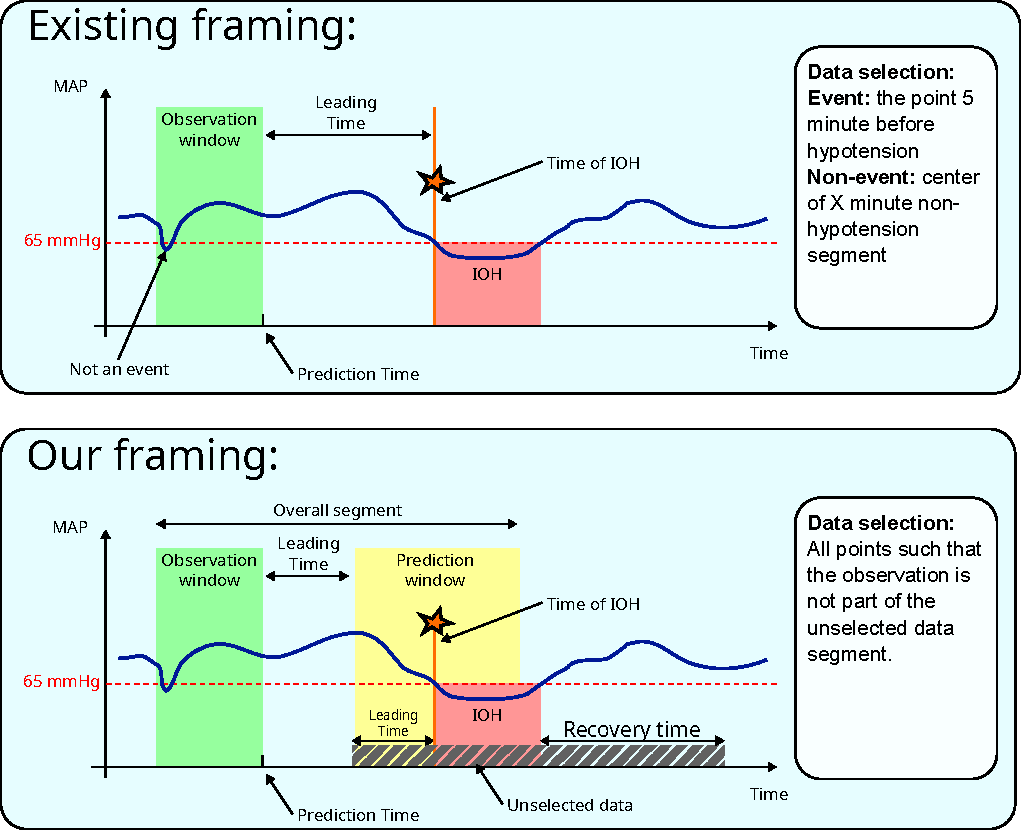
\includegraphics[width=\textwidth]{figures/framing.pdf}
    \caption{Illustration of the different framing of the problem.}
    \label{fig:framing}
\end{figure}

The parameters of our framing are the following:
\begin{itemize}
    \item The size of the observation window (first try with 3 minutes)
    \item The leading time (first try with 3 minutes)
    \item The size of the prediction window (first try with 7 minutes)
    \item The recovery time (first try with 15 minutes, should not change too much)
\end{itemize}

The impact of those parameters must be studied in this work or the followings.

\section{Data pre-processing}

The following flow chart describes the data selection of each segment of the data. 

\begin{figure}[h]
    \centering
    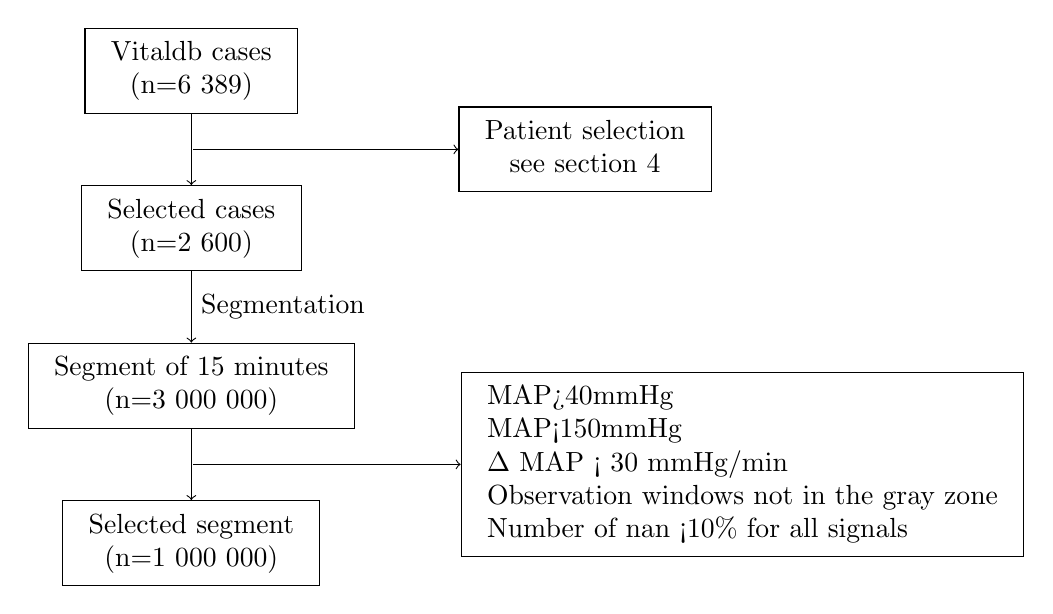
\begin{tikzpicture}
    \node (vdb) at (0, 0) [draw, rectangle, minimum width=2cm, minimum height=1cm] {\begin{tabular}{c} Vitaldb cases \\ (n=6 389) \end{tabular}};

    \node (cases) [draw, rectangle, below of=vdb, yshift= -1cm, minimum width=2cm, minimum height=1cm] {\begin{tabular}{c} Selected cases \\ (n=2 600) \end{tabular}};

    \node (features) [draw, rectangle, below of=cases, yshift= -1cm, minimum width=2cm, minimum height=1cm] {\begin{tabular}{c} Segment of 15 minutes \\ (n=3 000 000) \end{tabular}};

    \node (selected_features) [draw, rectangle, below of=features, yshift= -1cm, minimum width=2cm, minimum height=1cm] {\begin{tabular}{c} Selected segment \\ (n=1 000 000) \end{tabular}};

    \draw [->] (vdb) -- (cases) node (arrow1) [midway, xshift=-1mm] {};
    \draw [->] (cases) -- (features)node [midway, right] {Segmentation};
    \draw [->] (features) -- (selected_features) node (arrow3) [midway, xshift=-1mm] {};


    \node (patient_select) [draw, rectangle, right of=vdb, xshift= 4cm, yshift=-1cm, minimum width=2cm, minimum height=1cm] {\begin{tabular}{c} Patient selection \\ see section 4 \end{tabular}};
    \draw [<-] (patient_select) -- (arrow1);

    \node (feature_select) [draw, rectangle, right of=features, xshift= 6cm, yshift= -1cm, minimum width=2cm, minimum height=1cm] {\begin{tabular}{l} MAP>40mmHg \\ MAP<150mmHg \\ $\Delta$ MAP < 30 mmHg/min \\ Observation windows not in the gray zone \\ Number of nan <10\% for all signals \end{tabular}};
    \draw [<-] (feature_select) -- (arrow3);
\end{tikzpicture}
    \caption{Data pre-processing flow chart}
    \label{fig:preprocessing}
\end{figure}



\section{Evaluation}

To fairly evaluate the potential of our method against baseline and evaluate uncertainty on our results a Leave One Out Cross-Validation (LOOCV) is used \cite{meghnoudjSparseOptimalControlbased2024}. This method consist on partitioning the set of patient in $k$ distinct subset. Then to loops are nested, in the outer one a subset is leaved out before any training on the data and is used as a test set to assesse the performance of the method. In the inner one, a subset is leaved out to be used as a validation set for the hyperparameters tuning. This method is illustrated on Fig.~\ref{fig:loocv}.

\begin{figure}
    \centering
    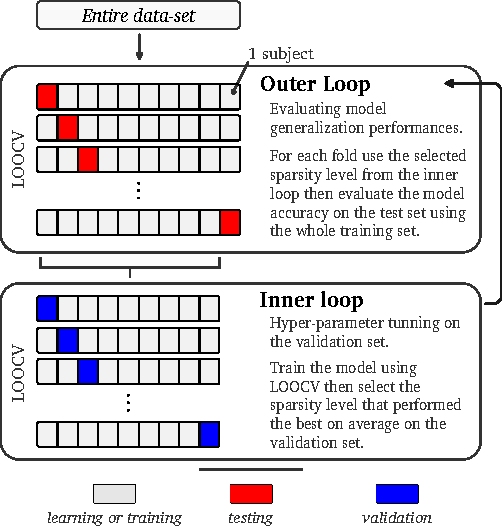
\includegraphics[width=0.7\textwidth]{figures/chap_1_NLOO.pdf}
    \caption{Illustration of Leave one out cross validation (from \cite{meghnoudjSparseOptimalControlbased2024})}
    \label{fig:loocv}
\end{figure}

In this work the metric used is the Aera Under the Receiver operating characteristic curve (AUC) \cite{masonAreasRelativeOperating2002a}. This curve evaluates the ability of a binary classifier at different threshold value and is usually used in medical field. It is the plot of the True Positive error against the False positive error (or sensitivity against 1 - specificity). The way to associate a $p$-value to this metric must be inestigated in \cite{masonAreasRelativeOperating2002a}.

\section{Baseline}

A fair baseline for the prediction of hypotension have been recently published in \cite{jacquet-lagrezePredictionIntraoperativeHypotension2022}. In this article they demonstrate that both linear extrapolation of MAP value and last value of MAP are good baseline for the prediction of hypotension. In this work, we used the last value of MAP as a baseline, as it is simplest to implement. \medskip

In fact after, testing on the dataset, it appears that the last value of the Diastolic Blood Pressure (DBP) is a better baseline than the last value of the MAP. As the DBP value is also available to the care team, it can also be condidered as a baseline. \medskip

\section{Proposed model}

To extract the features from the observation window, an exponential moving window (EMW) is used, as in \cite{lundbergExplainableMachinelearningPredictions2018}. Three different times constants are used for the EMW: 10s, 60s, 300s in order to capture different time scales. Both mean and standard deviation of the EMA are used as features. Thyis leads to a total of $6 \times 9 = 54$ time dependant feature plus 5 static features describing patient condition. \medskip

The model used is an Extreme Gradient Boosting (XGBoost) \cite{chenXGBoostScalableTree2016}. This model is a tree-based model that has been shown to be efficient in many medical applications \cite{chenXGBoostScalableTree2016}. The model is trained to predict the hypotension event in the prediction window. \medskip

The hyperparameters of the model are tuned using a grid search on the validation set of the LOOCV. The considered hyperparameters are the following:
\begin{itemize}
    \item The number of trees
    \item The maximum depth of the trees
    \item The learning rate
    \item The minimum child weight
\end{itemize}

\begin{figure}[h]
    \centering
    \newcommand{\errorband}[5][]{ % x column, y column, error column, optional argument for setting style of the area plot
% \pgfplotstableread{#2}\datatable
    % Lower bound (invisible plot)
    \addplot [draw=none, stack plots=y, forget plot] table [
        x={#3},
        y expr=\thisrow{#4}-2*\thisrow{#5},
        , col sep=comma
    ] {#2};

    % Stack twice the error, draw as area plot
    \addplot [draw=none, fill=gray!40, stack plots=y, area legend, #1] table [
        x={#3},
        y expr=4*\thisrow{#5},
        , col sep=comma
    ] {#2} \closedcycle;

    % Reset stack using invisible plot
    \addplot [forget plot, stack plots=y,draw=none] table [x={#3}, y expr=-(\thisrow{#4}+2*\thisrow{#5}), col sep=comma] {#2};
}

\readdef{../data/baseline_roc.csv}\mybaseline
\readarray*\mybaseline\myarraybaseline[-,\ncols]

\readdef{../data/xgboost_roc.csv}\myxgboost
\readarray*\myxgboost\myarrayxgboost[-,\ncols]

\begin{tikzpicture}

\definecolor{darkgray176}{RGB}{176,176,176}
\definecolor{lightgray204}{RGB}{204,204,204}
\definecolor{steelblue31119180}{RGB}{31,119,180}

\begin{axis}[
legend cell align={left},
legend style={
  fill opacity=0.8,
  draw opacity=1,
  text opacity=1,
  at={(0.97,0.03)},
  anchor=south east,
  draw=lightgray204
},
legend style={rounded corners=0.5mm, font=\footnotesize},
tick align=outside,
tick pos=left,
x grid style={darkgray176},
xlabel={1 - Specificity},
xmajorgrids,
xmin=0, xmax=1,
xtick style={color=black},
y grid style={darkgray176},
ylabel={Sensitivity},
ymajorgrids,
ymin=0, ymax=1,
ytick style={color=black}
]

\errorband[blue, opacity=0.2,forget plot]{../data/baseline_roc.csv}{fpr}{tpr}{tpr_std}
\errorband[orange, opacity=0.2,forget plot]{../data/xgboost_roc.csv}{fpr}{tpr}{tpr_std}

\addplot [semithick, blue] table[x=fpr, y=tpr, col sep=comma] {../data/baseline_roc.csv};
\addplot [semithick, orange] table[x=fpr, y=tpr, col sep=comma] {../data/xgboost_roc.csv};

\addlegendentry{baseline}
\addlegendentry{proposed model}
\addplot [semithick, black, dashed, forget plot]
table {%
0 0
1 1
};
\end{axis}

\end{tikzpicture}

    \caption{ROC curve of the model (AUC = mean $\pm$ std).}
    \label{fig:roc}
\end{figure}

The ROC curve of the model is shown in Fig.~\ref{fig:roc}, statistics of the given model compared to the baseline are given in Table~\ref{tab:result}.

\begin{table}
    \centering
    \scriptsize
    \begin{tabular}{l|ccccc}
\toprule
 & AUC & Sensitivity (\%) & Specificity (\%) & PPV (\%) & NPV (\%) \\
\midrule
Baseline &  0.72 [0.70, 0.74] &  64.80 [59.18, 70.43] &  71.64 [64.21, 79.08] &  14.70 [11.35, 18.05] &  96.45 [95.42, 97.47] \\
XGBoost &  0.79 [0.75, 0.83] &  71.72 [65.53, 77.90] &  71.83 [66.07, 77.58] &  16.09 [11.77, 20.41] &  97.15 [96.44, 97.86] \\
\bottomrule
\end{tabular}

    \caption{Performance of the baseline and the XGBoost model. The values are presented as mean [95\% CI]}
    \label{tab:result}
\end{table}

\section{Explainability}

To better understand the prediction of the model, the SHapley Additive exPlanations (SHAP) \cite{lundbergExplainableMachinelearningPredictions2018} are used. This method allows to explain the prediction of the model by attributing the contribution of each feature to the final prediction. Results for our model are shown in Fig.~\ref{fig:shap}.

% \begin{figure}
%     \centering
%     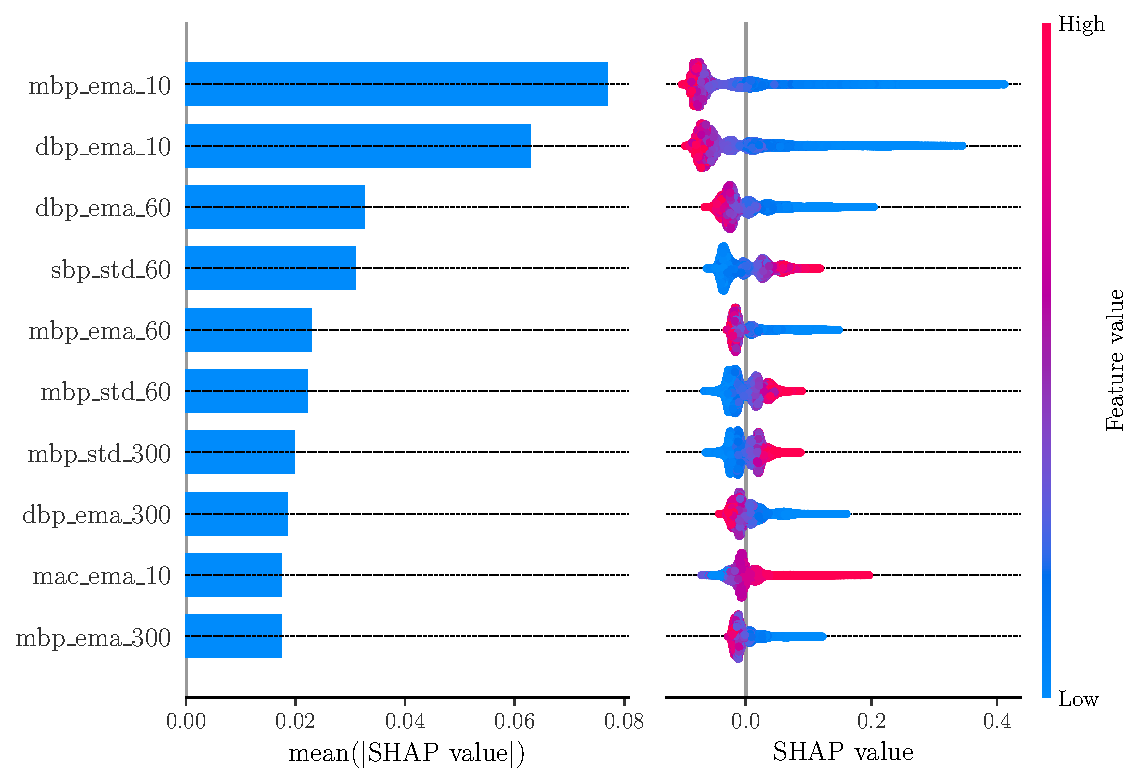
\includegraphics[width= 0.8\textwidth]{figures/shap_xgboost.pdf}
%     \caption{SHAP values of the model.}
%     \label{fig:shap}
% \end{figure}

\section{Statistical significance}

In this section we will consider the statistical significance of the results of the model against the baseline. Let's consider the nulle hypothesis:

\begin{equation}
    H_0: AUC_{model} = AUC_{baseline}
\end{equation}

Firs the $Z$ score must be computed:

\begin{equation}
    Z = \frac{AUC_{model} - AUC_{baseline}}{SE(AUC_{model} - AUC_{baseline})}
\end{equation}

where:

\begin{equation}
    SE(AUC_{model} - AUC_{baseline}) = \sqrt{VAR(AUC_{model}) + VAR(AUC_{baseline})}
\end{equation}

Assuming that the AUC are normally distributed and independent (Otherwhise the $Z$ score must be computed using the Welch-Satterthwaite equation). In our case the $Z$ score is 2.5. \medskip

The $p$-value can be computed using the $Z$ score. The $p$-value is the probability of observing a value of the test statistic as extreme as the one observed, assuming that the null hypothesis is true. The $p$-value is then compared to the significance level $\alpha$ (usually 0.05) to decide if the null hypothesis is rejected or not. \medskip

The $p$-value can be computed using the following formula:

\begin{equation}
    p = 2 \times (1 - \Phi(|Z|))
\end{equation}

where $\Phi$ is the cumulative distribution function of the standard normal distribution. We optain a p-value = 0.0001.\medskip



\bibliographystyle{ieeetr}
\bibliography{bibli}
 

\end{document}
